\documentclass[conference]{IEEEtran}
\IEEEoverridecommandlockouts

% Local XeTeX builds (e.g. Tectonic) cannot load the Type 1 Times that IEEEtran
% requests, and silently fall back to Latin Modern. Name the OpenType Times
% clone explicitly there. pdfLaTeX, Overleaf's default, skips this block.
\usepackage{iftex}
\ifXeTeX
  \usepackage{fontspec}
  \setmainfont{texgyretermes}[Extension=.otf, UprightFont=*-regular,
    BoldFont=*-bold, ItalicFont=*-italic, BoldItalicFont=*-bolditalic]
  \setmonofont{texgyrecursor}[Extension=.otf, UprightFont=*-regular,
    BoldFont=*-bold, ItalicFont=*-italic, BoldItalicFont=*-bolditalic]
\fi

\usepackage{cite}
\usepackage{amsmath,amssymb,amsfonts}
\usepackage{algorithm}
\usepackage{algpseudocode}
\usepackage{graphicx}
\usepackage{booktabs}
\usepackage{siunitx}
\sisetup{detect-all, per-mode=symbol}
\usepackage{textcomp}
\usepackage{xcolor}
\usepackage[hidelinks]{hyperref}
\usepackage{url}
\usepackage{tikz}
\usetikzlibrary{arrows.meta, positioning, fit, backgrounds}

\graphicspath{{figures/}}

% Numbers and tables generated by experiments/make_tables.py
% Auto-generated by experiments/make_tables.py -- do not edit.
% Every inline number in the paper resolves through these macros.
\newcommand{\AccOne}{85.1}
\newcommand{\AgeComparisons}{33\,223}
\newcommand{\AgeDayOne}{0.05}
\newcommand{\AgeDayOneMedian}{0.01}
\newcommand{\AgeFortnight}{16.2}
\newcommand{\AgeGrowth}{1.29}
\newcommand{\AgeMonth}{75.3}
\newcommand{\AgeMonthMedian}{13.69}
\newcommand{\AgeObjects}{60}
\newcommand{\AgeWeek}{4.3}
\newcommand{\AgeWeekMedian}{0.70}
\newcommand{\BaseSkew}{1.8}
\newcommand{\BestBudgetMode}{50\% of nights}
\newcommand{\BootResamples}{10\,000}
\newcommand{\BootStations}{6}
\newcommand{\BrightFamilies}{13}
\newcommand{\BrightHalfFitted}{24}
\newcommand{\BrightHalfLearned}{52}
\newcommand{\BrightHalfSphere}{14}
\newcommand{\BrightMaeFitted}{1.51}
\newcommand{\BrightMaeLearned}{0.83}
\newcommand{\BrightMaeSphere}{1.86}
\newcommand{\BrightObs}{17\,216}
\newcommand{\BrightSatMaeFitted}{1.93}
\newcommand{\BrightSatMaeLearned}{0.71}
\newcommand{\BrightSatMaeSphere}{2.43}
\newcommand{\BrightSats}{2709}
\newcommand{\BrightSplitDate}{2025-07}
\newcommand{\BrightStarlinkFitted}{1.57}
\newcommand{\BrightStarlinkLearned}{2.76}
\newcommand{\BrightTempEstFitted}{1.26}
\newcommand{\BrightTempEstLearned}{1.60}
\newcommand{\BrightTempEstSphere}{1.61}
\newcommand{\BrightTempMaeFitted}{1.99}
\newcommand{\BrightTempMaeLearned}{2.00}
\newcommand{\BrightTempMaeSphere}{2.31}
\newcommand{\BrightTempNewFitted}{3.29}
\newcommand{\BrightTempNewLearned}{2.69}
\newcommand{\BrightTempNewSphere}{3.53}
\newcommand{\BrightTempVisFitted}{0.67}
\newcommand{\BrightTempVisLearned}{0.51}
\newcommand{\BrightTempVisSphere}{0.54}
\newcommand{\BrightTestOnlyFamilies}{6}
\newcommand{\BrightVisFitted}{0.66}
\newcommand{\BrightVisLearned}{0.80}
\newcommand{\BrightVisSphere}{0.59}
\newcommand{\BtwWthRatio}{2.2}
\newcommand{\BudgetBlindClearRate}{13.9}
\newcommand{\BudgetClearRate}{23.1}
\newcommand{\BudgetGainClear}{37.6}
\newcommand{\BudgetGainClearHi}{80.4}
\newcommand{\BudgetGainClearLo}{3.1}
\newcommand{\BudgetGainClearPos}{0.98}
\newcommand{\BudgetGainEV}{19.0}
\newcommand{\BudgetGainEVHi}{24.9}
\newcommand{\BudgetGainEVLo}{9.2}
\newcommand{\BudgetOracleClear}{106.7}
\newcommand{\BudgetOracleEV}{46.0}
\newcommand{\BudgetRecoveredClear}{35}
\newcommand{\BudgetRecoveredEV}{41}
\newcommand{\BudgetTotal}{90}
\newcommand{\CallReduction}{23.7}
\newcommand{\CallsDense}{54\,864\,000}
\newcommand{\CallsFast}{2\,311\,148}
\newcommand{\CamEpochs}{30}
\newcommand{\CamFixedAcc}{72.6}
\newcommand{\CamFixedCorr}{0.856}
\newcommand{\CamFixedFone}{0.802}
\newcommand{\CamFixedFrac}{27.0}
\newcommand{\CamFixedIou}{0.669}
\newcommand{\CamGbmAcc}{96.8}
\newcommand{\CamGbmCorr}{0.998}
\newcommand{\CamGbmFone}{0.972}
\newcommand{\CamGbmFrac}{1.2}
\newcommand{\CamGbmIou}{0.945}
\newcommand{\CamImages}{400}
\newcommand{\CamThreshHi}{0.74}
\newcommand{\CamThreshLo}{0.74}
\newcommand{\CamThreshRange}{0.74 in every fold}
\newcommand{\CamTunedAcc}{92.3}
\newcommand{\CamTunedCorr}{0.994}
\newcommand{\CamTunedFone}{0.932}
\newcommand{\CamTunedFrac}{3.5}
\newcommand{\CamTunedIou}{0.873}
\newcommand{\CamUnetAcc}{95.8}
\newcommand{\CamUnetCorr}{0.998}
\newcommand{\CamUnetFone}{0.962}
\newcommand{\CamUnetFrac}{1.2}
\newcommand{\CamUnetIou}{0.927}
\newcommand{\Capacity}{3}
\newcommand{\ClearThreshold}{30}
\newcommand{\ClearThresholdEval}{30}
\newcommand{\CloudChennai}{88}
\newcommand{\CloudReduction}{0.209}
\newcommand{\DPBigMs}{285.3}
\newcommand{\DPBigN}{100\,000}
\newcommand{\DPOptimalPct}{100.00}
\newcommand{\DemoBright}{367}
\newcommand{\DemoCandidates}{87}
\newcommand{\DemoClear}{85}
\newcommand{\DemoDark}{1297}
\newcommand{\DemoGeometric}{12\,449}
\newcommand{\DemoHorizon}{7}
\newcommand{\DemoObjects}{635}
\newcommand{\DemoRuntime}{109.4}
\newcommand{\DemoScheduled}{26}
\newcommand{\DemoSunlit}{8093}
\newcommand{\DenseAos}{0.504}
\newcommand{\EpochMax}{13.04}
\newcommand{\EpochMean}{0.55}
\newcommand{\EpochMedian}{0.42}
\newcommand{\EpochPninety}{0.95}
\newcommand{\EpochUnderOne}{90.2}
\newcommand{\EvalDays}{60}
\newcommand{\EvalEnd}{2026-08-23}
\newcommand{\EvalObjects}{300}
\newcommand{\EvalStart}{2026-06-25}
\newcommand{\EvalStations}{6}
\newcommand{\EvalStationsWord}{six}
\newcommand{\ForecastDays}{60}
\newcommand{\ForecastEnd}{2026-08-23}
\newcommand{\ForecastStart}{2026-06-25}
\newcommand{\GAGenerations}{120}
\newcommand{\GAPct}{99.67}
\newcommand{\GAPopulation}{60}
\newcommand{\GASites}{6}
\newcommand{\GASlowdown}{38\,922}
\newcommand{\GreedyBestPct}{99.95}
\newcommand{\GreedyElevMin}{9.4}
\newcommand{\GreedyElevOptPct}{62.7}
\newcommand{\GreedyElevPct}{95.39}
\newcommand{\GreedyGain}{\ensuremath{-}60.0}
\newcommand{\GreedyValueMin}{85.9}
\newcommand{\GreedyValuePct}{99.95}
\newcommand{\GreedyWorstPct}{95.07}
\newcommand{\HistBudgetClear}{33.2}
\newcommand{\HistBudgetEV}{19.0}
\newcommand{\HistQuotaClear}{9.2}
\newcommand{\HistQuotaEV}{1.7}
\newcommand{\HistTightClear}{75.9}
\newcommand{\HssOne}{0.347}
\newcommand{\HssPersistence}{0.206}
\newcommand{\HssSeven}{0.114}
\newcommand{\HssThree}{0.289}
\newcommand{\InterceptMax}{0.70}
\newcommand{\InterceptMin}{0.07}
\newcommand{\JaccardDurOnly}{0.86}
\newcommand{\JaccardExtreme}{0.70}
\newcommand{\JaccardMid}{0.89}
\newcommand{\JaccardNinety}{0.70}
\newcommand{\MaeOne}{0.193}
\newcommand{\MaePersistence}{0.212}
\newcommand{\Missed}{4}
\newcommand{\NCatalogue}{635}
\newcommand{\NMatched}{1761}
\newcommand{\NPasses}{1801}
\newcommand{\NSats}{635}
\newcommand{\PassCorr}{0.41}
\newcommand{\ProviderN}{308}
\newcommand{\ProviderObjects}{52}
\newcommand{\ProviderTcaMax}{1.82}
\newcommand{\ProviderTcaMean}{0.041}
\newcommand{\ProviderTcaMedian}{0.00}
\newcommand{\ProviderTcaPninetyfive}{0.176}
\newcommand{\PythonVersion}{3.13.5}
\newcommand{\QuotaGainClear}{\ensuremath{-}0.2}
\newcommand{\QuotaGainClearHi}{3.5}
\newcommand{\QuotaGainClearLo}{\ensuremath{-}11.6}
\newcommand{\QuotaGainClearPos}{0.46}
\newcommand{\QuotaGainEV}{\ensuremath{-}1.5}
\newcommand{\QuotaGainEVHi}{2.0}
\newcommand{\QuotaGainEVLo}{\ensuremath{-}2.7}
\newcommand{\QuotaOracleClear}{31.6}
\newcommand{\QuotaOracleEV}{12.0}
\newcommand{\QuotaRawEV}{\ensuremath{-}9.2}
\newcommand{\RawBudgetClear}{29.9}
\newcommand{\RawBudgetEV}{8.0}
\newcommand{\RawQuotaClear}{\ensuremath{-}5.5}
\newcommand{\Recall}{99.78}
\newcommand{\ScaleDays}{7}
\newcommand{\ScaleObjects}{635}
\newcommand{\ScalePasses}{12\,438}
\newcommand{\ScaleSchedMs}{2.1}
\newcommand{\ScaleSeconds}{104.4}
\newcommand{\SchedTrials}{2000}
\newcommand{\SgpVersion}{2.27}
\newcommand{\SkillStations}{7}
\newcommand{\SkillStationsWord}{seven}
\newcommand{\SkyfieldAos}{0.060}
\newcommand{\SkyfieldElev}{0.0034}
\newcommand{\SkyfieldTca}{0.055}
\newcommand{\SkyfieldTcaMax}{0.293}
\newcommand{\SlopeChennai}{0.56}
\newcommand{\SlopeMax}{0.61}
\newcommand{\SlopeMin}{0.17}
\newcommand{\StructureDays}{30}
\newcommand{\TightBudget}{45}
\newcommand{\TightClearRate}{28.1}
\newcommand{\TightGainClear}{55.0}
\newcommand{\TightGainClearHi}{144.5}
\newcommand{\TightGainClearLo}{24.7}
\newcommand{\TightGainClearPos}{1.00}
\newcommand{\TightGainEV}{19.2}
\newcommand{\TrainDays}{90}


\begin{document}

\title{SkyPass: Exact Weather-Aware Scheduling of\\Satellite Passes for Small Ground Stations}

\author{\IEEEauthorblockN{Rohith Prem S}
\IEEEauthorblockA{\textit{Student}\\
\textit{Department of Computer Science and Engineering}\\
\textit{Saveetha Engineering College}\\
Chennai, India\\
rohithprem91@gmail.com}
\and
\IEEEauthorblockN{Dr.\ R. Selvakumar}
\IEEEauthorblockA{\textit{Associate Professor}\\
\textit{Department of Artificial Intelligence and Machine Learning}\\
\textit{Saveetha Engineering College}\\
Chennai, India\\
selvakumarr@saveetha.ac.in}
}

\maketitle

\begin{abstract}
Observation planning at a small ground station is presently distributed across
unconnected tools: one predicts passes, another evaluates optical visibility,
cloud conditions are checked manually, and conflicts between overlapping passes
are resolved by the operator. Cloud cover is the least well handled of these,
since conventional predictors enumerate passes without reference to it. This
paper presents SkyPass, an integrated planner that carries a catalogue of
orbital elements through propagation, pass extraction, visibility scoring,
cloud-forecast integration and exact conflict resolution to an executable
timetable. Pass extraction uses coarse bracketing with bisection refinement,
achieving \SkyfieldTca~s mean agreement with an independent implementation while
requiring \CallReduction$\times$ fewer propagator evaluations than a dense scan.
Conflict resolution is formulated as weighted interval scheduling under a
nightly observing budget and solved exactly by a dynamic program whose running
time grows linearly with the number of candidate passes and the nightly limit;
it matched exhaustive search on all \SchedTrials~randomised instances tested. Forecast
skill is verified against ERA5 reanalysis at \SkillStationsWord{} stations and
scheduling value at \EvalStationsWord{}, over \EvalDays~days. The principal finding
is that forecast value is determined by the decision the forecast informs: a
station required to observe every night obtains no benefit, whereas one able to
select its observing nights improves realised yield by \BudgetGainEV\% (expected
value) and \BudgetGainClear\% (clear-sky count). Calibrating the forecast
against reanalysis raises the gain in every regime tested; under a nightly quota
the uncalibrated forecast performs worse than disregarding weather.
\end{abstract}

\begin{IEEEkeywords}
satellite pass prediction, SGP4, ground station scheduling, interval scheduling,
forecast calibration, optical observation
\end{IEEEkeywords}

% ===========================================================================
\section{Introduction}

Small ground stations, such as university laboratories, amateur-radio clubs and
individual optical observers, face a recurring planning problem. Several hundred
satellites are potentially observable and over a week generate thousands of
passes, of which only a few dozen merit the operator's time, and the station can
attend to one object at a time.

Existing tools address only parts of this problem. Pass predictors compute rise
and set times from two-line elements (TLEs) and the SGP4
propagator~\cite{vallado2022fundamentals, acciarini2025sgp4}, and some add an
illumination test so that optical observers are not shown daylight passes. A few
applications display a weather indication beside a pass, but to our knowledge
none allow the forecast to \emph{rank} passes or drive a scheduling decision,
and none resolve conflicts between overlapping passes.

The treatment of weather is the more consequential omission. At the site used as
a running example (Chennai, India, \ang{12.92}\,N), the mean observed cloud
cover over optically viable passes was \CloudChennai\%, under which most
geometrically favourable passes are not observable. A predictor ranking passes
by culmination elevation will nonetheless recommend an overcast night. The
scheduling omission is less apparent. Once several satellites are tracked
their passes overlap, and a single-aperture station must select among them. The
literature addressing this problem does so from the operator side of the link,
as spacecraft tasking and satellite range scheduling, formulated as mathematical
programs or addressed with metaheuristics and learning methods~\cite{li2023srsp,
song2023cluster, ou2023drl, wang2024avns, wang2021agile}. Such formulations
impose constraints a small station does not have, and solver dependencies it
cannot justify.

This paper shows that the small-station problem admits a substantially simpler
exact formulation, and that the treatment of weather is what improves realised
outcomes. The contributions are: an integrated pipeline accounting for the
passes removed by each physical constraint; a validated pass extractor; exact
capacity-constrained conflict resolution requiring neither a solver nor a
metaheuristic; a weather claim verified against ERA5
reanalysis~\cite{hersbach2020era5}; two negative results, namely that
weather-awareness yields no benefit under a fixed nightly quota and that the
uncalibrated forecast degrades performance there; and a measured element-set
error budget over \AgeComparisons{} aged comparisons.

% ===========================================================================
\section{Related Work}

SGP4 and its two-line element sets remain the standard
basis for rapid satellite position prediction~\cite{vallado2022fundamentals,
acciarini2025sgp4}. Accuracy is limited by the element sets rather than the
propagator: TLE-derived positions carry errors that grow with element-set age,
as measured against on-board GPS~\cite{kovar2022tle} and estimated
statistically~\cite{curzi2021tle}.

Whether a satellite is \emph{seen} depends on
illumination and photometry, not only geometry. Standard treatments use a
conical Earth-shadow model~\cite{vallado2022fundamentals} and a diffuse-sphere
phase function for apparent magnitude~\cite{fankhauser2023brightness}, and
recent megaconstellation brightness work has refined
these~\cite{mallama2021starlink, lawler2022visibility}.

Satellite range scheduling is an oversubscribed
combinatorial problem~\cite{li2023srsp}, usually approached with multi-objective
optimisation, metaheuristics or reinforcement learning~\cite{petelin2021ground,
ou2023drl}. Earth observation scheduling is a large adjacent
literature~\cite{wang2021agile, eddy2021mis}, in which cloud cover appears as an
uncertainty to be hedged during imaging tasking~\cite{wang2020robust,
wang2021robust}, although always on the \emph{operator} side. Where the
underlying structure is single-machine interval selection, exact polynomial
algorithms exist: weighted interval scheduling is a textbook dynamic
program~\cite{cormen2022introduction}, and harder members of the family continue
to attract exact methods~\cite{muir2023interval}.

Professional observatories schedule around
weather using queue schedulers that re-plan as conditions
change~\cite{zhang2024grris, xie2024astrosa}, but assume an institutional
software stack and on-site sky monitoring. Forecast verification and forecast
value are mature fields~\cite{brown2021met, turner2022hrrr}, and statistical
post-processing is essential before a forecast drives a
decision~\cite{vannitsem2021postprocessing}. To our knowledge this machinery has
not been applied to observer-side pass planning.

% ===========================================================================
\section{System Design}
\label{sec:design}

SkyPass is a five-stage pipeline (Fig.~\ref{fig:arch}). Each stage is a pure
function of the preceding one, so any stage may be ablated independently, which
is the mechanism by which the weather claim is evaluated.

\begin{figure}[htbp]
\centering
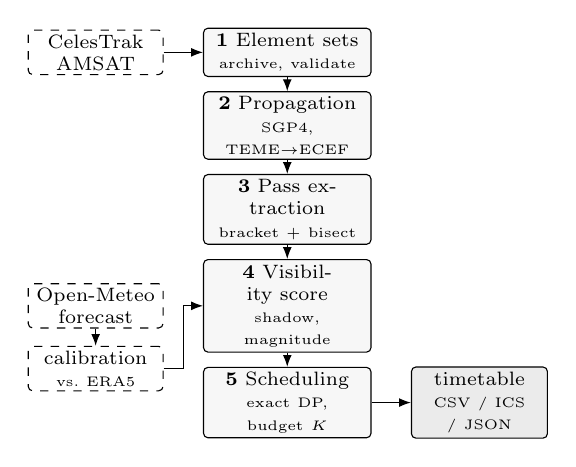
\begin{tikzpicture}[
  font=\scriptsize,
  node distance=1.8mm,
  box/.style={draw, rounded corners=1.6pt, align=center, inner sep=1.8pt,
              minimum height=4.6mm, text width=20mm, fill=black!3},
  src/.style={draw, dashed, rounded corners=1.6pt, align=center,
              inner sep=1.6pt, minimum height=4.2mm, text width=16mm,
              fill=black!0},
  result/.style={draw, rounded corners=1.6pt, align=center,
                 inner sep=1.8pt, minimum height=4.6mm, text width=16mm,
                 fill=black!8},
  ar/.style={-{Latex[length=1.5mm]}, thin},
]
\node[box] (tle)   {\textbf{1} Element sets\\\tiny archive, validate};
\node[box, below=of tle]  (prop) {\textbf{2} Propagation\\\tiny SGP4, TEME$\to$ECEF};
\node[box, below=of prop] (pass) {\textbf{3} Pass extraction\\\tiny bracket + bisect};
\node[box, below=of pass] (score){\textbf{4} Visibility score\\\tiny shadow, magnitude};
\node[box, below=of score](sched){\textbf{5} Scheduling\\\tiny exact DP, budget $K$};

\node[src, left=5mm of tle]   (ct)  {CelesTrak\\AMSAT};
\node[src, left=5mm of score] (om)  {Open-Meteo\\forecast};
\node[src, below=2.2mm of om] (cal) {calibration\\\tiny vs.\ ERA5};

\node[result, right=5mm of sched] (ics) {timetable\\\tiny CSV / ICS / JSON};

\draw[ar] (ct)   -- (tle);
\draw[ar] (tle)  -- (prop);
\draw[ar] (prop) -- (pass);
\draw[ar] (pass) -- (score);
\draw[ar] (score)-- (sched);
\draw[ar] (om)   -- (cal);
\draw[ar] (cal.east) -- ++(2.5mm,0) |- (score.west);
\draw[ar] (sched)-- (ics);
\end{tikzpicture}
\caption{SkyPass pipeline. The cloud forecast is calibrated against reanalysis
before it is allowed to influence the score; the scheduler then resolves
conflicts exactly under the station's nightly observing budget.}
\label{fig:arch}
\end{figure}

\subsection{Element sets, propagation and pass extraction}
Element sets are fetched from CelesTrak~\cite{celestrak}, checksum-validated,
deduplicated per NORAD identifier keeping the newest epoch, and \emph{archived
under the date of retrieval}: CelesTrak serves only current elements, so without
a local archive a published prediction cannot be repeated. Sets whose epoch age
exceeds $\tau_\mathrm{max}$ are rejected.

Positions come from the reference SGP4 implementation. The TEME vector is
rotated to ECEF by Greenwich mean sidereal time and converted to topocentric
azimuth, elevation and range on the WGS-84 ellipsoid. Polar motion is neglected,
being below \SI{15}{\metre} at the surface and far under the SGP4 error budget.
Atmospheric refraction~\cite{stuhl2021refraction} is reported but not applied to
the horizon mask, so results do not depend on assumed surface conditions.

Because cost is dominated by propagator calls, pass extraction is designed to
minimise them (Algorithm~\ref{alg:passes}). Elevation is sampled on a coarse
grid to \emph{bracket} horizon crossings; within a pass elevation is smooth and
unimodal, so a sign change of $\varepsilon(t) - \varepsilon_\mathrm{mask}$
between adjacent samples brackets exactly one crossing. Each bracket is refined
by bisection to \SI{0.1}{\second}, and culmination by golden-section search. The
coarse step is $P/240$ bounded to \SIrange{5}{30}{\second}, so short-period
orbits, whose passes are shortest, are sampled most finely.

\begin{algorithm}[htbp]
\caption{Pass extraction for one object}
\label{alg:passes}
\begin{algorithmic}[1]
\Require element set $\sigma$, window $[t_0,t_1)$, mask $\varepsilon_m$,
         tolerance $\delta$
\State $h \gets \max(5,\min(\Delta_\mathrm{max}, P(\sigma)/240))$
\State $t \gets t_0$; \; $e_\mathrm{prev} \gets \varepsilon(\sigma,t)$;
       \; $a \gets \textbf{nil}$
\While{$t < t_1$}
  \State $t' \gets \min(t+h,\,t_1)$; \; $e \gets \varepsilon(\sigma,t')$
  \If{$e_\mathrm{prev} < \varepsilon_m \le e$}
     \State $a \gets \textsc{Bisect}(t,t',\varepsilon_m,\text{rising},\delta)$
  \ElsIf{$e_\mathrm{prev} \ge \varepsilon_m > e$ \textbf{and} $a \ne$ \textbf{nil}}
     \State $l \gets \textsc{Bisect}(t,t',\varepsilon_m,\text{setting},\delta)$
     \State $c \gets \textsc{GoldenMax}(a,l,\delta)$
     \State \textbf{emit} pass $(a,c,l)$; \; $a \gets \textbf{nil}$
  \EndIf
  \State $t \gets t'$; \; $e_\mathrm{prev} \gets e$
\EndWhile
\end{algorithmic}
\end{algorithm}

\subsection{Visibility scoring}
Each pass receives a score $S \in [0,1]$ combining a geometric quality term with
multiplicative gates:
\begin{equation}
S = \underbrace{\left(w_e f_e + w_d f_d\right)}_{\text{geometry}}
    \cdot \; f_m \cdot f_s ,
\label{eq:score}
\end{equation}
where $f_e = \min(\varepsilon_\mathrm{max}/\ang{60},1)$ and
$f_d = \min(T/\SI{480}{\second},1)$ saturate culmination elevation and duration,
$f_m$ is a photometric factor and $f_s$ a sky-condition factor.

The multiplicative form is deliberate: an eclipsed pass or one in a bright sky
scores zero irrespective of its geometry, and expected cloud scales the score
down in proportion, which an additive score cannot represent. For optical work
the object must be sunlit and
the observer in darkness; Earth shadow uses the dual-cone
construction~\cite{vallado2022fundamentals}, and apparent magnitude follows the
standard diffuse-sphere relation~\cite{fankhauser2023brightness, mccants}
\begin{equation}
m = m_\mathrm{std} + 5\log_{10}\!\frac{d}{\SI{1000}{\kilo\metre}}
    - 2.5\log_{10} F(\psi),
\label{eq:mag}
\end{equation}
with $F(\psi) \propto (\pi-\psi)\cos\psi + \sin\psi$ normalised to $F(0)=1$. In
radio mode the illumination and photometric terms are dropped.

\subsection{Weather integration and calibration}
\label{sec:calib}
The sky factor is $f_s = 1 - \hat{c}$, where $\hat{c}$ is the expected cloud
fraction at culmination, interpolated linearly between hourly samples. Crucially
$\hat{c}$ is \emph{not} the raw forecast, which is heavily over-confident as a
predictor. We fit
\begin{equation}
\hat{c} = \mathbb{E}[c \mid c_f] = a + b\,c_f
\label{eq:calib}
\end{equation}
by least squares on a window that \emph{ends before} the period being planned,
restricted to local night hours, and clip $\hat{c}$ to $[0,1]$. The slope $b$
quantifies the strength of the
signal: $b \approx 1$ indicates that the forecast may be used directly, whereas
$b \approx 0$ indicates that it carries little information, in which case the
calibrated value converges toward site climatology, the appropriate fallback. For the threshold value model the planner instead weights
each pass by the calibrated probability of clear sky,
$P(c \le \theta \mid c_f)$, estimated in ten forecast bins on the same window
and shrunk toward the site's base rate with 20 pseudo-observations, so each value
model is paired with the planner that maximises its expectation.

\subsection{Conflict resolution}
\label{sec:sched}
A single-aperture station observes one object at a time and requires a setup gap
$g$ between targets, so selecting the best mutually compatible subset of passes
is weighted interval scheduling. Writing $v_j = S_j \pi_j$ for the value of pass
$j$ (score times mission priority), indexing passes $1,\dots,n$ by finish time
and letting $p(j)$ be the largest $i<j$ compatible with $j$ ($0$ if none), the
textbook recurrence~\cite{cormen2022introduction} gives the exact optimum in
$O(n\log n)$.

This formulation alone is insufficient: left unconstrained, a station observes
every candidate, so weather-awareness has no selection to perform. Operational
stations are limited by operator and instrument time, so we impose a capacity
budget of $K$ observations per night, extending the recurrence with a
cardinality dimension:
\begin{equation}
\mathrm{OPT}[j][k] = \max\bigl(\mathrm{OPT}[j\!-\!1][k],\;
      v_j + \mathrm{OPT}[p(j)][k\!-\!1]\bigr),
\label{eq:dp}
\end{equation}
with $\mathrm{OPT}[0][k]=\mathrm{OPT}[j][0]=0$. This is exact. The table has one entry for each of the $n$
candidate passes and each count up to the nightly limit $K$, and each entry is
filled in constant time, so after the sort the cost is $O(nK)$: doubling either
the candidates or the limit doubles the work. Observing nights are disjoint
in time, so applying the budget per night and solving each night independently
remains exact. Nights are defined in local solar time so that an evening and the
small hours that follow belong to the same session.

% ===========================================================================
\section{Experimental Setup}
\label{sec:setup}

The catalogue comprises \NCatalogue{} unique objects from CelesTrak GP groups,
checksum-validated and deduplicated per object. Seven stations span distinct
cloud climatologies: Chennai and Bengaluru (monsoon), Leh (high-altitude arid),
Tucson (desert), Singapore (equatorial), and Reykjav\'ik and Svalbard (maritime
polar). Unless stated otherwise, the mask is \ang{10}, the dark-sky threshold
\ang{-6}, and the setup gap \SI{5}{\minute}.

All three weather products come from Open-Meteo~\cite{openmeteo}: the
operational forecast; archived past forecasts
at lead times of 1--7 days; and ERA5 reanalysis~\cite{hersbach2020era5} as
verification truth. The archive endpoint has to be pinned to the ERA5 model:
its default best-match series \emph{is}, for recent dates, the archived
forecast, and verifying against it reports a spurious skill of 1.0.

Timing is checked against a brute-force \SI{1}{\second} dense scan and against
Skyfield~\cite{skyfield}, which shares only the certified SGP4 core and
implements time scales, frames and event finding independently. All runs are
single-threaded, under Python~\PythonVersion{} with \texttt{sgp4}~\SgpVersion{}
on a commodity laptop.

% ===========================================================================
\section{Results}

\subsection{Pass-prediction accuracy and cost}
\label{sec:accuracy}

Table~\ref{tab:accuracy} compares SkyPass against both references over
\NSats{} objects and \NMatched{} matched passes.

\begin{table}[t]
\caption{Pass-timing agreement over the full catalogue (635 objects, 1761 matched passes, 24\,h horizon). Values in seconds.}
\label{tab:accuracy}
\centering
\begin{tabular}{lcccc}
\toprule
& \multicolumn{2}{c}{vs.\ 1\,s dense scan} & \multicolumn{2}{c}{vs.\ Skyfield} \\
\cmidrule(lr){2-3}\cmidrule(lr){4-5}
Quantity & mean & p95 & mean & p95 \\
\midrule
$|\Delta t_\mathrm{AOS}|$ & 0.504 & 0.954 & 0.060 & 0.157 \\
$|\Delta t_\mathrm{TCA}|$ & 0.248 & 0.476 & 0.055 & 0.110 \\
$|\Delta t_\mathrm{LOS}|$ & 0.502 & 0.956 & 0.059 & 0.156 \\
$|\Delta \varepsilon_\mathrm{max}|$ (deg) & 0.0008 & 0.0022 & 0.0034 & 0.0102 \\
\bottomrule
\end{tabular}
\end{table}


Against Skyfield, mean agreement is \SkyfieldAos~s on acquisition and
\SkyfieldTca~s on culmination. The apparent \DenseAos~s ``deviation'' from the
dense scan is not SkyPass error: a \SI{1}{\second} grid locates a crossing only
to within its own step, so it lags the true crossing by a mean of
\SI{0.5}{\second}. The refined estimator is thus more accurate than the
brute-force reference it is conventionally compared against. The cost
difference is large: \CallsFast{} propagator evaluations against \CallsDense{},
a factor of \CallReduction. Detection recall is \Recall\%, the residual being
very short grazing transits that peak barely above the mask.

\subsection{Element-set limits on prediction accuracy}
\label{sec:elements}

Sub-second numerical agreement is meaningful only if the orbital elements
support that precision. In the operational catalogue the median element-set age
was \EpochMedian~days (\EpochUnderOne\% under one day). CelesTrak and AMSAT
element sets differ by a mean of \ProviderTcaMean~s in culmination over
\ProviderN{} matched passes, but the median difference is \ProviderTcaMedian~s:
the two providers largely redistribute the same upstream sets, so this bounds
redistribution differences rather than independent orbit determination.

To measure
decay with staleness we obtained historical element sets for \AgeObjects{}
low-Earth objects, took the freshest set before a target night as reference, and
re-predicted the same passes from progressively older sets, giving
\AgeComparisons{} aged comparisons (Fig.~\ref{fig:tleage}).

\begin{figure}[htbp]
\centering
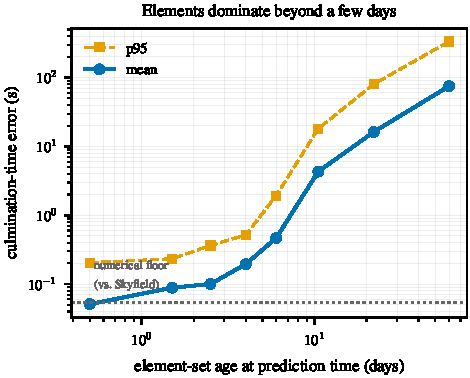
\includegraphics[width=0.85\columnwidth]{fig_tle_age.pdf}
\caption{Culmination-time error against element-set age, over
\AgeComparisons{} aged comparisons. The dotted line is the numerical agreement
with Skyfield. Fresh elements land on that floor; by a week the mean is nearly
two orders of magnitude above it.}
\label{fig:tleage}
\end{figure}

Within a day of epoch the elements contribute \AgeDayOne~s of culmination error,
the same order as the \SkyfieldTca~s numerical agreement of
Section~\ref{sec:accuracy}, so neither term dominates at that age. Degradation
is then sharply super-linear and heavy-tailed: a mean of \AgeWeek~s (median
\AgeWeekMedian~s) at 7--14 days, \AgeFortnight~s at 14--30, and \AgeMonth~s
(median \AgeMonthMedian~s) beyond a month. The design consequence is that a 5--7
day staleness cutoff is appropriate for timing-critical work, beyond which the
elements rather than the algorithm set achievable accuracy, and that daily
element refresh is the single largest lever on prediction accuracy.

\subsection{Skill of the cloud forecast}
\label{sec:forecast}

Weather-aware planning is justified only if the forecast is informative at the
lead times over which an observer plans. Archived forecasts were verified
against ERA5 across all seven stations over \ForecastDays{} days, scoring the
operational binary decision of whether a given hour is sufficiently clear to
observe at a \ClearThreshold\% cloud threshold. Accuracy alone is misleading
when clear hours are rare, so we report the Heidke skill score, a
chance-corrected measure in wide use for categorical forecast
verification~\cite{ebert2022rare}.

Skill decays steadily with lead time, from HSS \HssOne{} at one day to
\HssThree{} at three days and \HssSeven{} at seven. The one-day forecast
outperforms both naive baselines (persistence \HssPersistence, climatology 0 by
construction), but by five to seven days it no longer does. A weather-aware
planner should therefore run on a rolling short horizon and re-plan daily. Skill is also strongly site-dependent, the
spread between stations being comparable to the decay with lead time and lowest
at the two Indian monsoon stations, Chennai reaching zero skill beyond four
days. The expected benefit of weather-awareness is thus a local property rather
than a universal constant.

\subsection{Value of weather-aware scheduling}
\label{sec:value}

Five planners select from an identical candidate set, drawn from
\EvalObjects{} objects, at each of \EvalStationsWord{} stations over \EvalDays{}
days (Svalbard has no observable passes), and every
timetable is scored against ERA5. Since the
valuation of a clouded observation is a modelling choice, we report both an
\emph{expected value} model, $\sum_j v_j (1-c_j)$, and a \emph{threshold} model,
$\sum_j v_j \mathbb{1}[c_j \le \theta]$ with $\theta = \ClearThresholdEval\%$.

\begin{figure}[htbp]
\centering
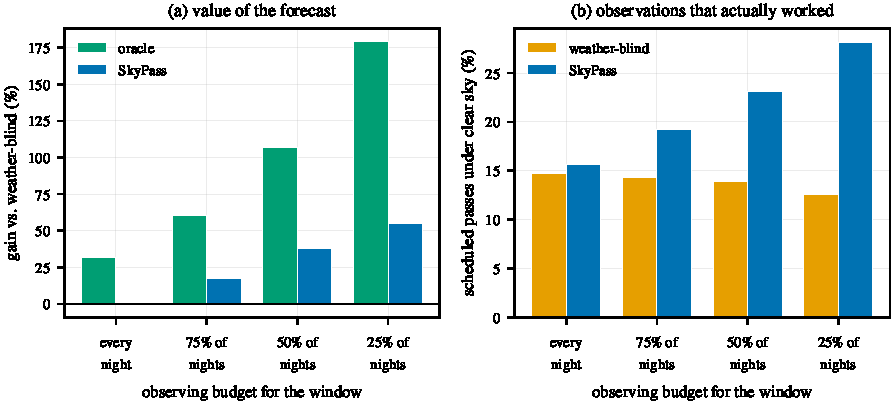
\includegraphics[width=0.95\columnwidth]{fig_budget_modes.pdf}
\caption{Weather-awareness is worth nothing to a station obliged to observe
every night, and a great deal to one that may choose its nights. (a) Gain over
the weather-blind exact planner, threshold value model; the oracle plans with
the observed cloud. (b) Share of scheduled passes under clear sky.}
\label{fig:budget}
\end{figure}

Under a fixed nightly quota the forecast yields no benefit: SkyPass gains
\QuotaGainEV\% under the expected-value model and \QuotaGainClear\% under the
threshold model, against oracle headroom of \QuotaOracleEV\% and
\QuotaOracleClear\% respectively, and the station-bootstrap intervals of both
gains include zero. This is not because the forecast is
uninformative: at the candidate-pass timestamps, forecast and observed cloud
correlate at $r = \PassCorr$, and the clearest-forecast decile does identify
clearer skies, reducing observed cloud by $\CloudReduction$.

The limitation is that a nightly quota permits the planner only to
\emph{reorder passes within a night}, which two measured properties render
ineffective. Cloud is strongly autocorrelated over the few hours a session
spans, the between-night standard deviation of observed cloud being
$\BtwWthRatio\times$ the within-night value; and pass quality varies more than
sky conditions do, the ninetieth-percentile pass carrying $\BaseSkew\times$ the
mean weather-free value. Since the score is a product, selecting for clear sky
requires surrendering base value, an exchange that is unfavourable where quality
is the more variable factor.

Given the same nightly cap together with a budget for the window, so that it may
\emph{skip} a night, the result reverses (Fig.~\ref{fig:budget}): the choice of
which nights to use is a day-scale decision, the scale at which the forecast
retains skill. Under the budget permitting observation on \BestBudgetMode{}
(\BudgetTotal{} observations across the window), SkyPass improves realised yield
by \BudgetGainEV\% under the expected-value model and \BudgetGainClear\% under
the threshold model (95\% intervals \BudgetGainEVLo--\BudgetGainEVHi\% and
\BudgetGainClearLo--\BudgetGainClearHi\%), recovering \BudgetRecoveredEV\% and
\BudgetRecoveredClear\% of the attainable oracle gains. The fraction of
scheduled passes falling under clear sky rises from \BudgetBlindClearRate\% to
\BudgetClearRate\%, and tightening the budget to a quarter of the nights raises
the threshold-model gain to \TightGainClear\%.

\begin{figure}[htbp]
\centering
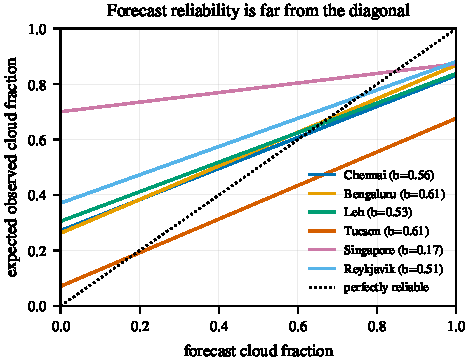
\includegraphics[width=0.85\columnwidth]{fig_calibration.pdf}
\caption{Fitted forecast reliability. A perfectly reliable forecast would lie on
the dotted diagonal; the fitted slopes are far below one, so the raw model field
over-states its own discrimination.}
\label{fig:calib}
\end{figure}

Calibration raises the gain in every regime. Under the quota,
supplying the model cloud field directly to the score costs \QuotaRawEV\%
relative to disregarding weather; under the half budget the raw field still
helps (\RawBudgetEV\% and \RawBudgetClear\%) but less than the calibrated one.
Fig.~\ref{fig:calib} indicates the cause: fitted slopes lie between \SlopeMin{}
and \SlopeMax{} and intercepts between \InterceptMin{} and \InterceptMax{}, so
clear forecasts are followed by more cloud than predicted and cloudy ones by
less. Calibration \eqref{eq:calib} shrinks the forecast toward climatology in
proportion to its demonstrated reliability.

Repeating the evaluation with epoch-correct geometry, that is, with the element
set current on each night, raises the threshold-model gain under the
quota from \QuotaGainClear\% to \HistQuotaClear\% and at a quarter budget from
\TightGainClear\% to \HistTightClear\%, but lowers it at the half budget from
\BudgetGainClear\% to \HistBudgetClear\%, the expected-value gain there being
unchanged at \HistBudgetEV\%. Back-propagated geometry therefore does not
inflate the result systematically, although it is not uniformly conservative.

\subsection{Conflict resolution in practice}
\label{sec:schedresults}

On \SchedTrials{} randomised instances small enough to enumerate exhaustively,
the dynamic program matched the exhaustive optimum in \DPOptimalPct\% of cases.
Greedy selection \emph{by the score itself} attains \GreedyValuePct\% of the
optimum on average, so the dynamic program offers little average-case
improvement over it; its advantage is that it is exact, has negligible cost, and
exhibits no adverse case. The rules an operator typically applies perform
markedly worse (Fig.~\ref{fig:sched}), since they optimise a proxy rather than
the objective: selection by highest culmination attains \GreedyElevPct\% on
average, is optimal in only \GreedyElevOptPct\% of instances, and falls to
\GreedyElevMin\% in the worst case generated.

\begin{figure}[htbp]
\centering
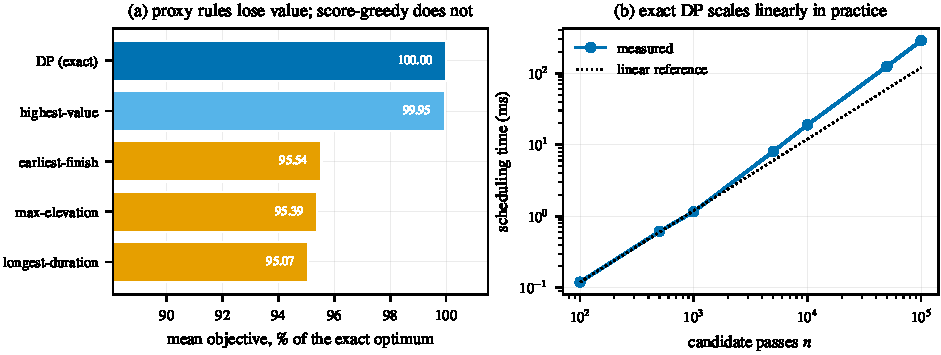
\includegraphics[width=0.95\columnwidth]{fig_scheduler.pdf}
\caption{(a) Greedy heuristics attain less than the exact dynamic program.
(b) Scheduling time grows linearly in practice and remains negligible at
catalogue scale.}
\label{fig:sched}
\end{figure}

On real candidate sets, an order-based genetic algorithm of the type common in
the satellite-tasking literature (population \GAPopulation, \GAGenerations{}
generations) attains \GAPct\% of the optimum but requires approximately
\GASlowdown$\times$ more time, a ratio that depends on that search budget. Once
the problem is recognised as interval scheduling, an exact polynomial solution
is available and a metaheuristic is unnecessary. Scheduling is in any case not the bottleneck, the dynamic
program handling \DPBigN{} candidates in \DPBigMs~ms against the seconds to
minutes required for propagation.

\subsection{End-to-end behaviour}
\label{sec:pipeline}

The funnel is steep and physically interpretable (Fig.~\ref{fig:funnel}): at the
demonstration site, \DemoGeometric{} geometric passes reduce to \DemoSunlit{}
sunlit, \DemoDark{} with the observer in darkness, \DemoBright{} bright enough
to detect, \DemoCandidates{} above the score floor once forecast cloud is
weighted in, and \DemoScheduled{} scheduled. A weather-blind tool would present
the operator with the earlier, substantially larger counts. Per-station runs also provide a physical consistency check:
Svalbard (\ang{78.2}\,N) returns the largest number of geometric and sunlit
passes of any station, yet \emph{zero} optically observable passes, since in
late August the Sun does not fall below the \ang{-6} dark-sky threshold there.

\begin{figure}[htbp]
\centering
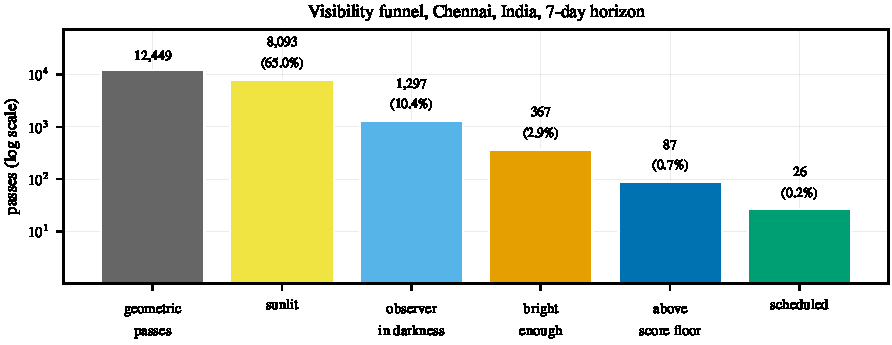
\includegraphics[width=0.85\columnwidth]{fig_funnel.pdf}
\caption{Visibility funnel for the demonstration station: of \DemoGeometric{}
geometric passes over \DemoHorizon{} days, \DemoScheduled{} survive to the
timetable. Cloud enters the score as a continuous weight rather than a hard
cut, so the penultimate stage is the score floor.}
\label{fig:funnel}
\end{figure}

Planning \DemoObjects{} objects over \DemoHorizon{} days takes \DemoRuntime~s
single-threaded, dominated by propagation, which scales linearly in objects and
horizon. The timetable is also stable against the score weights: varying $w_e$
from 0.3 to 0.7 leaves a Jaccard overlap of at least \JaccardMid{} with the
default timetable, falling to \JaccardNinety{} once elevation dominates
($w_e \ge 0.9$) and to \JaccardDurOnly{} with duration alone. Within the
moderate range the physical constraints, not the weighting, govern the
outcome.

% ===========================================================================
\section{Discussion and Limitations}
\label{sec:discussion}

Cloud cover is an imperfect proxy for observing conditions: total cloud
fraction on a reanalysis grid cell of order \SI{25}{\kilo\metre} describes a
line of sight only coarsely, and transparency, seeing, cloud height and aerosol
are not modelled. A local all-sky camera could supply a better nowcast, to
which the calibration of Section~\ref{sec:calib} would apply unchanged, and
sub-hourly skill would let a quota-constrained planner discriminate within a
night. Neither value model captures partial credit; a station with a specific
instrument would be better served by its own value function, which the
scheduler accepts unchanged.

The gains pool \EvalStationsWord{} stations and \EvalDays{} nights in one
season. Their 95\% intervals come from a bootstrap that resamples whole stations
(\BootResamples{} draws); with so few clusters they are approximate and probably
too narrow, and the calibrated-minus-raw difference was not tested separately.

We assume one instrument observing one object at a time;
multiple apertures or a station network break the interval-scheduling structure
and would require a different algorithm. Photometry is approximate, since
\eqref{eq:mag} models every object as a diffuse sphere, so the magnitude gate is
an ordering rather than a prediction. The ageing measurement is single-season
and restricted to low Earth orbit, where drag-driven decay dominates.

% ===========================================================================
\section{Conclusion}

SkyPass integrates pass prediction, optical visibility analysis, cloud-forecast
reasoning and exact conflict resolution into a single planner suitable for
deployment at a small ground station, producing a timetable that exports
directly to a calendar or a rotator controller. Pass extraction agrees with an
independent implementation to \SkyfieldTca~s while requiring
\CallReduction$\times$ fewer propagator calls than dense sampling, and conflict
resolution is exact at negligible computational cost.

Two weather-related findings are of particular relevance to the design of such
systems. First, a forecast does not by itself improve performance: it is
informative about which \emph{nights} merit observation and much less so for
ranking passes within a night, where cloud is autocorrelated and pass quality
varies substantially more than sky conditions. A planner under a fixed nightly
quota cannot exploit that information and gains nothing, whereas given a budget
it may allocate selectively the same forecast yields \BudgetGainEV\% (expected
value) and \BudgetGainClear\% (clear-sky count). Second, calibration against
reanalysis raises the gain in every regime tested, and under a quota it is the
difference between a loss and break-even. Both findings should carry over to
other small facilities, though only one setting is tested here: the value of a
forecast is a property of the decision it informs. The implementation and
experiment scripts are released under the MIT licence.

\section*{Acknowledgements}
The authors thank the Department of Artificial Intelligence and Machine Learning
and the Department of Computer Science and Engineering, Saveetha Engineering
College, Chennai, for their support of this work. This work uses public orbital
element sets from CelesTrak and AMSAT, and weather data from Open-Meteo
including ECMWF forecasts and ERA5 reanalysis. A generative AI assistant
(Claude, Anthropic) was used to edit and restructure the text of all sections
and to write the scripts that build the manuscript; the authors reviewed all
such output and take responsibility for the content.

\bibliographystyle{IEEEtran}
\bibliography{refs}

\end{document}
